% ------------------------------------------------------------------------------------
\vspace{5mm}
{\color{lightgray} \hrule}
\begin{enumerate}
	\item Sean $x_i \sim G a(\alpha, \beta)$; $i=1,2, \ldots, n$. Simular datos $x_i$ con $\alpha=3$ y $\beta=100$ considerando los casos $n=5$ y $40$.
	
	Con $\alpha \sim \mathrm{U}(1,4), \beta \sim \exp (1)$ distribuciones a priori, se tiene la posterior
	\begin{equation} \label{eq:1}
		 f(\alpha, \beta \mid \bar{x}) \propto \frac{\beta^{n \alpha}}{\Gamma(\alpha)^n} r_1^{\alpha-1} e^{-\beta\left(r_2+1\right)} \cdot \mathbbm{1}_{(1 \leq \alpha \leq 4)} \cdot \mathbbm{1}_{(\beta>1)}
	\end{equation}
	con
	\begin{equation} \label{eq:2}
		r_2= \sum_{i=1}^n x_i \text { y } r_1=\prod_{i=1}^n x_i
	\end{equation}
	
	En ambos casos, grafica los contornos para visualizar dónde está concentrada la posterior. Utilizar la propuesta
	\begin{equation} \label{eq:3}
		q\left(\left.\binom{\alpha_p}{\beta_p} \right\rvert\,\binom{\alpha}{\beta}\right)=\binom{\alpha}{\beta}+\binom{\varepsilon_1}{\varepsilon_2}
	\end{equation}
	donde
	\begin{equation}
		\binom{\varepsilon_1}{\varepsilon_2} \sim \mathcal{N}_2\left( \binom{0}{0}, \left(
		\begin{array}{cc}
			\sigma_1^2 & 0 \\
			0 & \sigma_2^2
		\end{array}
		\right)\right).
	\end{equation}
\end{enumerate}

\textcolor{BrickRed}{\it Respuesta:}

En el archivo \textcolor{mediumblue}{ejercicio1\_tarea7.py} se implementa la función \textit{METROPOLIS\_HASTINGS\_SIM()} la cual aplica el algoritmo Metropolis-Hastings para propuestas simétricas simulando una cadena de Markov en $\mathbb{R}^n$ y toma los siguientes argumentos:
\begin{itemize}
	\item La función objetivo $f$ (en este caso es la posterior \eqref{eq:1}).
	\item La distribución propuesta $q_{gen}$ (en este caso es la propuesta \eqref{eq:3}).
	\item El valor inicial $x_0$ (en este caso es $(\alpha, \beta)$ con $\alpha \sim \mathrm{U}(1,4), \beta \sim \exp (1)$).
	\item El número de iteraciones del algoritmo (casi siempre se usa $N = 10,000$).
\end{itemize}

Regresa la cadena de Markov simulada en $\mathbb{R}^n$ y usa el criterio de aceptación: si $y_t$ es la propuesta dada por $q_{gen}(\cdot|x_t)$ en $x_t$, entonces se acepta $y_t$ con probabilidad $\rho(x_t, y_t)$ con
\begin{equation}
	\rho(x,y) = \min\left\{1, \frac{f(y)}{f(x)} \right\}
\end{equation}
(en este caso, $\frac{q(x|y)}{q(y|x)} = 1$ ya que la propuesta es simétrica) y se rechaza con probabilidad $1-\rho(x_t, y_t)$. A continuación, se define la función \textit{SIMULAR\_GAMMA()}, la cual hace las simulaciones $x_i \sim G a(\alpha, \beta)$; $i=1,2, \ldots, n$

Después, se define la función posterior \eqref{eq:1} llamada \textit{posterior()}, y la función \textit{propuesta\_gen()} dada por \eqref{eq:3} la cual, como vimos en clase, es simétrica. Dentro de la función \textit{posterior()} se aplicó el logaritmo a los términos para evitar desbordamientos numéricos.

Finalmente:
\begin{itemize}
	\item Se simulacion $x_i \sim G a(\alpha = 3, \beta=100)$; $i=1,2, \ldots, n$ para los casos $n_{1}=5$ y $n_{2}=40$.
	\item Se dio el punto inicial $x_0=(\alpha_0, \beta_0)$ con $\alpha_0 \sim \mathrm{U}(1,4), \beta_0 \sim \exp (1)$. Tal punto resultó ser: $(3.886, 1.007)$.
	\item Se aplicó el algoritmo Metropolis-Hastings para generar las cadenas correspondientes para $n_1$ y $n_2$ usando $N=10,000$ iteraciones.
	\item Se usaron los parámetros de varianza de la propuesta $\sigma_1=0.1$ y $\sigma_2=10$ (se comenta más de esta elección al final).
	\item Se generaron los histogramas resultantes de $\alpha$ y $\beta$ para ambs casos y se graficaron los contornos para visualizar la concentración de la posterior.
\end{itemize}

Se obtuvieron los siguientes resultados: para $n_1=5$ se obtuvo una tasa de aceptación del $18.45\%$ y el promedio de la cadena para cada parámetro resultó ser: $(1.163, 6.006)$ Mientras que para $n_2=40$ se obtuvo una tasa de aceptación del $21.42\%$ y el promedio de la cadena para cada parámetro resultó ser: $(1.131, 19.920)$. Los histogramas resultantes se encuentran en la figura siguiente:
\begin{figure}[h]
	\centering
	\begin{minipage}{0.495\textwidth}
		\centering
		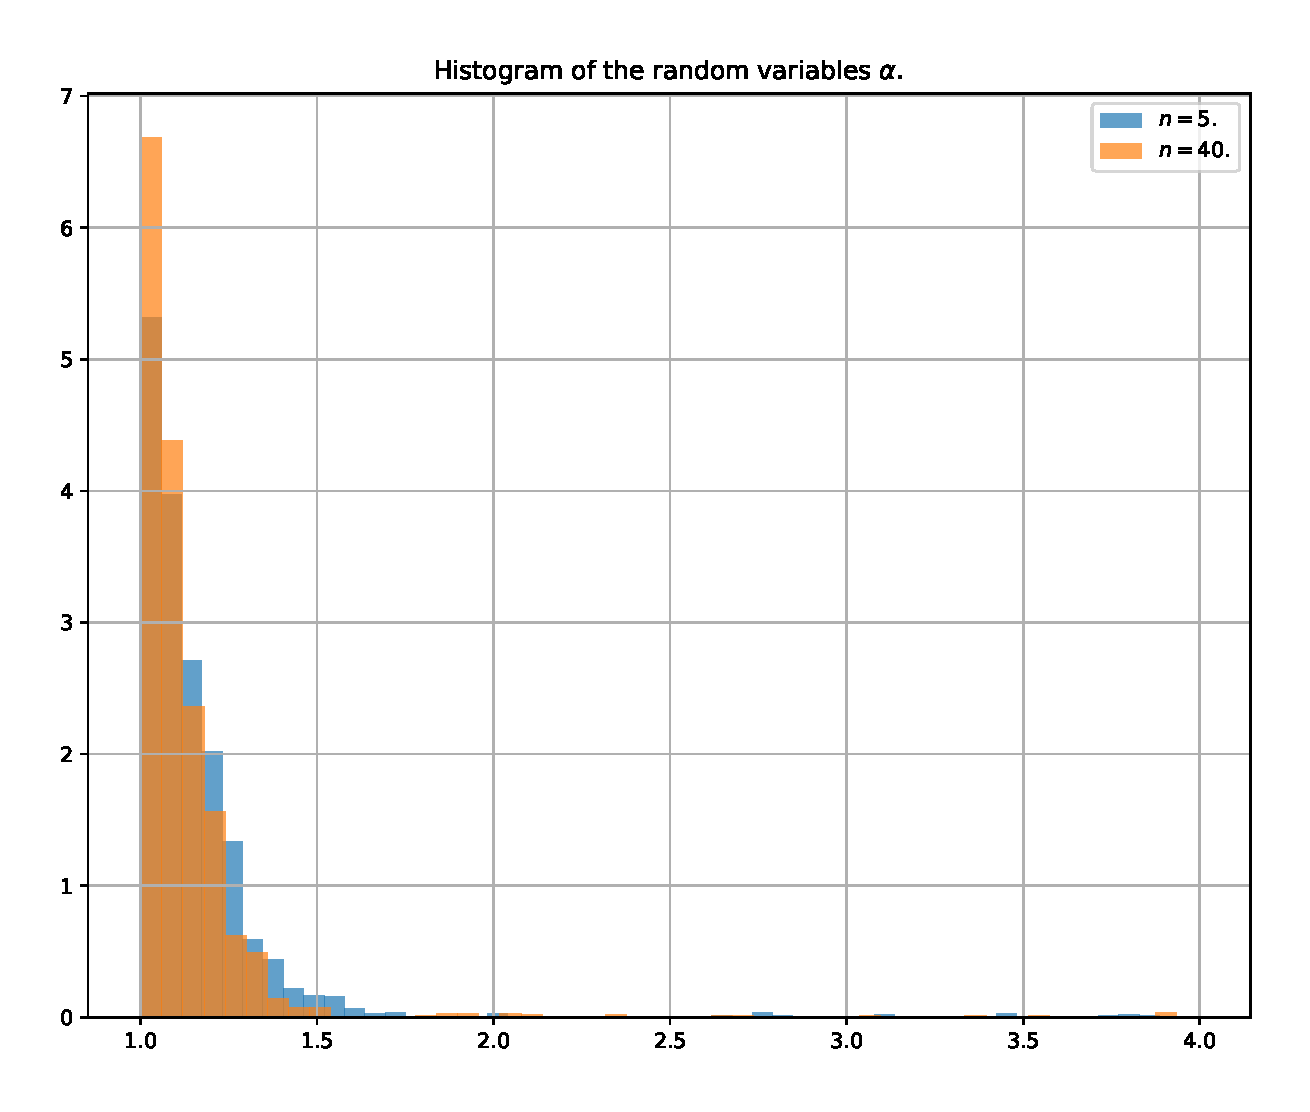
\includegraphics[width=\textwidth]{IMAGENES/ex1/histogram_n5.pdf}
		\caption{$\alpha$.}
	\end{minipage}
	\hfill
	\begin{minipage}{0.495\textwidth}
		\centering
		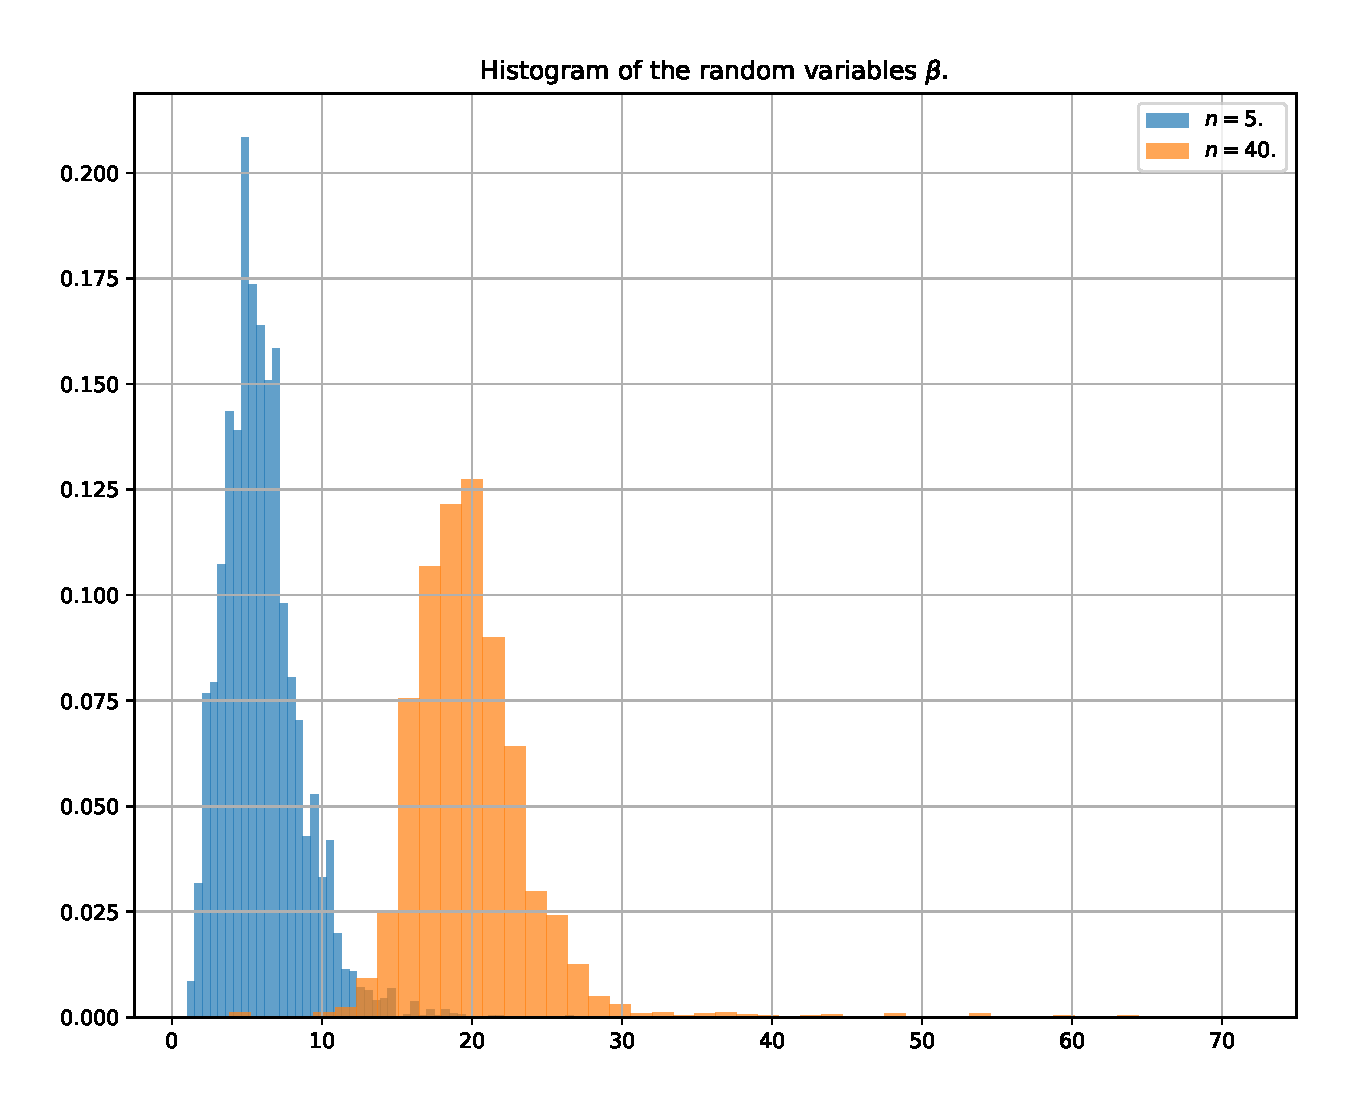
\includegraphics[width=\textwidth]{IMAGENES/ex1/histogram_n40.pdf}
		\caption{$\beta$.}
	\end{minipage}
\end{figure}

El gráfico de contornos es:
\begin{figure}[h!]
	\centering
	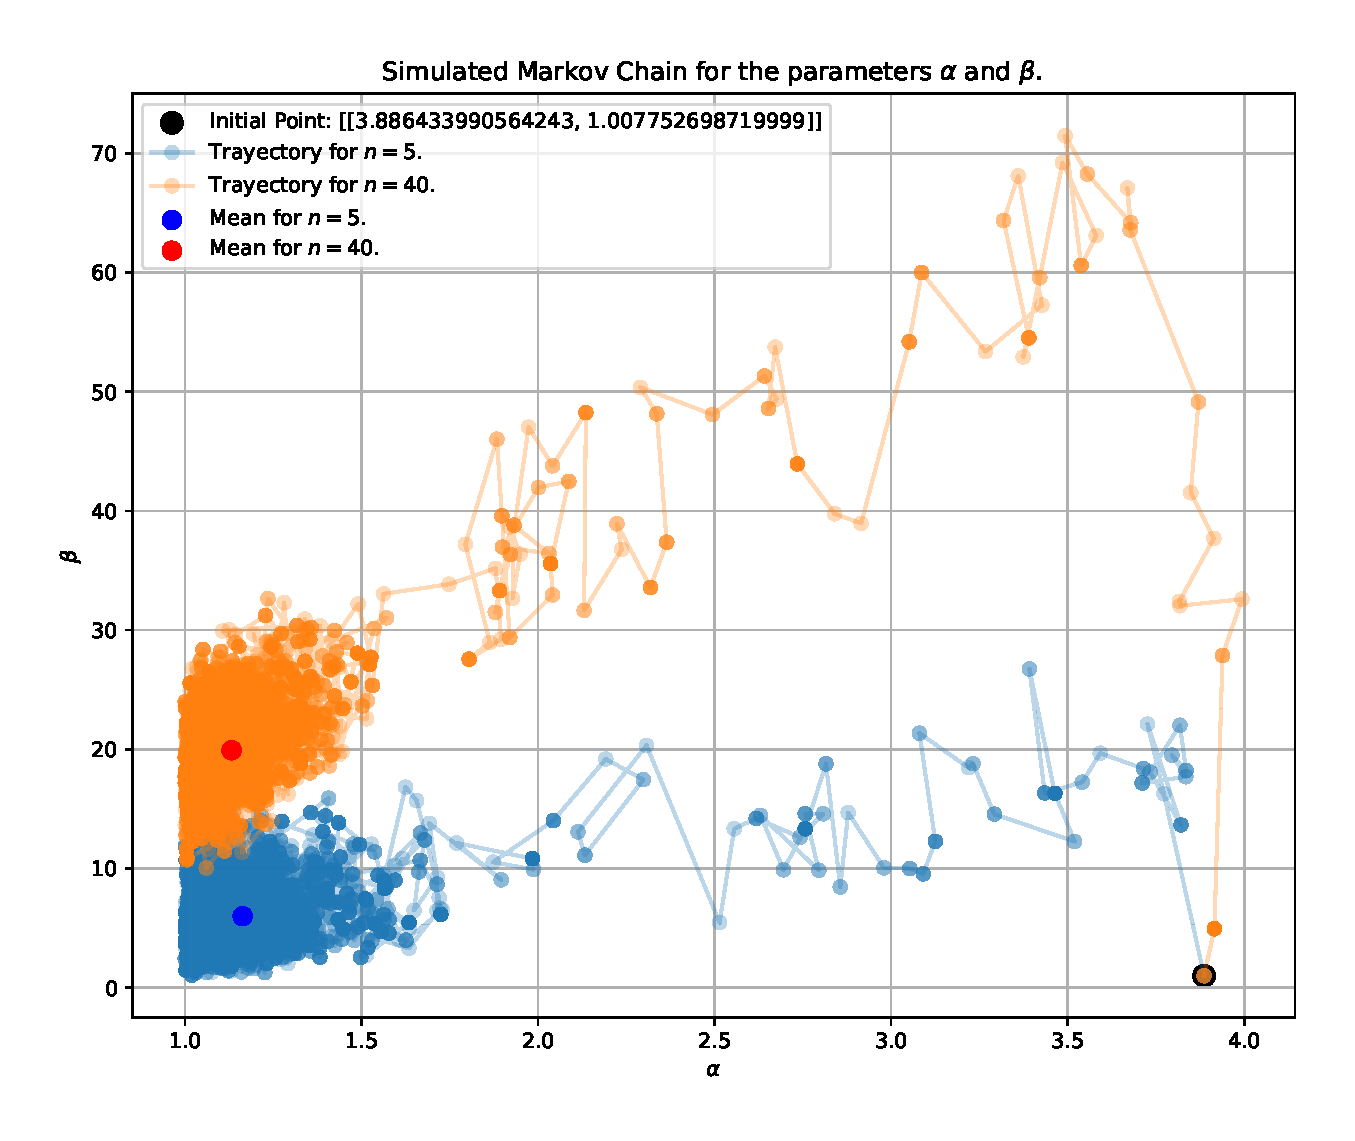
\includegraphics[width=0.76\textwidth]{IMAGENES/ex1/trayectory_ex1.pdf}
\end{figure}

Nótese que los valores promedio de las cadenas generadas se encuentran los puntos rojo y azul del gráfico anterior. En este caso particular, se puede ver que existe más varianza en el eje vertical, esto debido a que se tomó $\sigma_2$ $100$ veces mayor que $\sigma_1$. Otro ejemplo con varianzas distintas es:
\begin{figure}[h!]
	\centering
	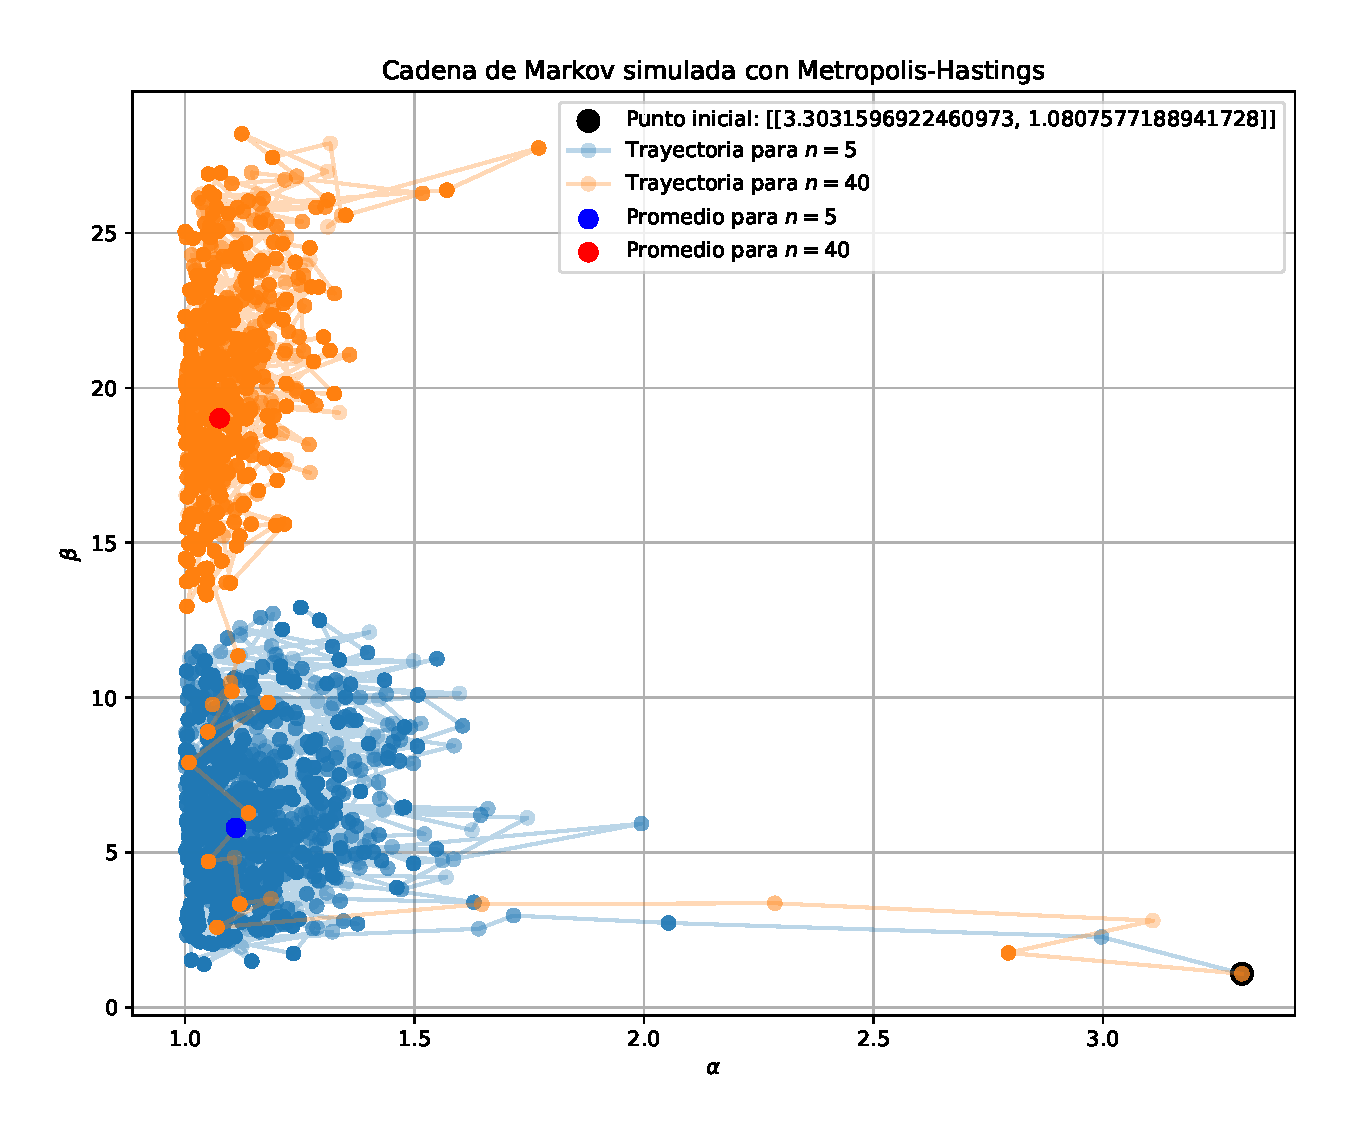
\includegraphics[width=0.76\textwidth]{IMAGENES/ejer12.pdf}
\end{figure}

En este último caso, se usó $\sigma_1=\sigma_2=1$. Sin importar el punto inicial, las varianzas elegidas o llevar el número de iteraciones a valores muy grandes, el algoritmo siempre terminaba alrededor de los mismos puntos, lo cual no corresponde con lo esperado ya que sabemos que los valores usados para generar las muestras fueron $\alpha=3$ y $\beta=100$. Incluso se varió $n$ para tener muestras más grandes y el resultado era similar (aunque sí hacía crecer los promedios de la cadena) o se volvía imposible de obtener debido a que el cálculo de $r_1$ causaba muchas indeterminaciones.